\chapter{Γεννήτρια Χωροχρονικών Δεδομένων}

\section{Αποθήκευση πηγαίων χωρικών δεδομένων}

Η γεννήτρια χωροχρονικών δεδομένων χρησιμοποιεί πραγματικά σημεία ενδιαφέροντος στο χάρτη ως πηγή χωρικών δεδομένων, όπως αυτά εμφανίζονται στη διαδικτυακή υπηρεσία 
συστημάτων προτάσεων (recommendation systems), TripAdvisor \cite{7}. Τα σημεία αυτά αναγνωρίζονται από τις γεωγραφικές συντεταγμένες τους καθώς και τη 
διεύθυνση τους στο χάρτη. Επίσης, συνοδεύονται από βαθμολογίες και κριτικές, οι οποίες έχουν γίνει από χρήστες της υπηρεσίας TripAdvisor. Το πλήθος των  
διαθέσιμων σημείων ενδιαφέροντος για τη δημιουργία της γεννήτριας χωροχρονικών δεδομένων ανέρχεται σε σύνολο 136409 σημείων, τα οποία προέκυψαν από αρχείο 
μεγέθους 13GB. Για την αποθήκευσή τους χρησιμοποιήθηκε 
η σχεσιακή βάση δεδομένων PostgreSQL. Το σχήμα της βάσης περιλαμβάνει δύο πίνακες, έναν για τα σημεία ενδαφέροντος και τα χαρακτηριστικά τους και έναν για τις κριτικές και 
βαθμολογίες που έχουν γίνει στα σημεία αυτά. 

\begin{figure}[H]
  \centering
  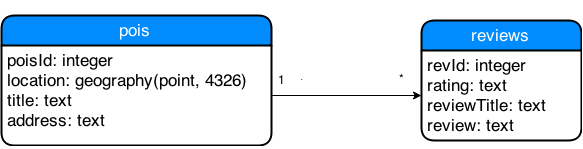
\includegraphics[width=0.7\textwidth]{figures/schema.png}
  \caption{Σχήμα βάσης δεδομένων για τα πηγαία χωρικά δεδομένα}
\end{figure}

Πιο αναλυτικά, ο πίνακας για τα σημεία ενδιαφέροντος περιέχει τα εξής γνωρίσματα:

\begin{itemize}
 \item poisId: αναγνωριστικός ακέραιος αριθμός του σημείου ενδιαφέροντος, κύριο κλειδί.
 \item location: οι γεωγραφικές συντεταγμένες του σημείου. Χρήση του γεωγραφικού τύπου δεδομένων ο οποίος υποστηρίζεται από την επέκταση PostGIS της PostgreSQL.
 \item title: η ονομασία του σημείου.
 \item address: η διεύθυνση του σημείου.
\end{itemize}

Ένα σημείο ενδιαφέροντος μπορεί να έχει πολλές κριτικές, γι'αυτό και οι δύο πίνακες συνδέονται με σχέση 1 προς πολλά. Ο πίνακας για τις κριτικές περιέχει τα εξής 
γνωρίσματα:

\begin{itemize}
 \item revId: αναγνωριστικός ακέραιος αριθμός του σημείου ενδιαφέροντος στο οποίο αντιστοιχεί η κριτική, εξωτερικό κλειδί.
 \item rating: βαθμολογία του σημείου σε κλίμακα ακεραίων 1 έως 5.
 \item reviewTitle: ο τίτλος της κριτικής για το σημείο.
 \item review: το κείμενο της κριτικής για το σημείο.
\end{itemize}

Μετά την αποθήκευση όλων των διαθέσιμων χωρικών δεδομένων αναθέτουμε ένα ευρετήριο τύπου B-tree στο γνώρισμα poisId του πίνακα pois και στο γνώρισμα revId του πίνακα 
reviews. Επίσης, δημιουργούμε ένα ευρετήριο τύπου GiST στο γνώρισμα location του πίνακα pois. Με τις δομές αυτές θα μπορεί να γίνει αποδοτικά η αναζήτηση 
εγγραφών ως προς τους αναγνωριστικούς τους αριθμούς αλλά και ως προς την τοποθεσία ενός σημείου ενδιαφέροντος. 

\section{Οντότητες γεννήτριας}

Με το ακόλουθο διάγραμμα κλάσης περιγράφονται οι οντότητες που χρησιμοποιούνται στην περιγραφή του σχεδιασμού της γεννήτριας.

\begin{figure}[H]
  \centering
  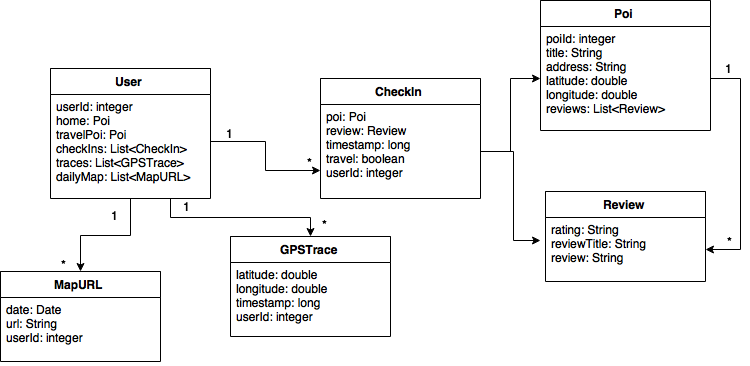
\includegraphics[width=0.9\textwidth]{figures/class_diagram.png}
  \caption{Διάγραμμα κλάσης οντοτήτων γεννήτριας}
\end{figure}

\subsection{Χρήστης - User}

Ο χρήστης που παράγεται από τη γεννήτρια έχει τα εξής γνωρίσματα:

\begin{itemize}
 \item userId: ακέραιος αριθμός αναγνωριστικός του χρήστη
 \item home: η κατοικία του χρήστη, η οποία είναι τύπου Poi, δηλαδή σημείου ενδιαφέροντος
 \item travelPoi: η κεντρική τοποθεσία του τρέχοντος ταξιδιού, η οποία είναι επίσης τύπου Poi
 \item checkIns: λίστα με όλες τις επισκέψεις (checkIn) τις οποίες πραγματοποίησε ο χρήστης κατά το χρονικό διάστημα εφαρμογής της γεννήτριας
 \item traces: λίστα με τα στίγματα δορυφόρου (GPSTrace) από τις όλες τις τροχιές στο χάρτη, τις οποίες πραγματοποίησε 
 ο χρήστης κατά το χρονικό διάστημα εφαρμογής της γεννήτριας
 \item dailyMap: λίστα με τους ημερήσιους στατικούς χάρτες (MapURL), οι οποίοι απεικονίζουν τις αντίστοιχες ημερήσιες τροχιές του χρήστη στο χάρτη.
\end{itemize}

\subsection{Επίσκεψη - Check-in}

Μία επίσκεψη ενός χρήστη σε ένα σημείο ενδιαφέροντος έχει τα ακόλουθα γνωρίσματα:

\begin{itemize}
 \item poi: το σημείο ενδιαφέροντος (Poi) στο οποίο γίνεται η επίσκεψη.
 \item review: η κριτική που άφησε ο χρήστης για το συγκεκριμένο σημείο στην αντίστοιχη επίσκεψη.
 \item timestamp: η χρονική στιγμή στην οποία έγινε η επίσκεψη σε αναπαράσταση αριθμού τύπου long
 \item travel: δυαδική τιμή η οποία υποδηλώνει αν η αντίστοιχη επίσκεψη γίνεται κατά τη διάρκεια ταξιδιού.
 \item userId: ο χρήστης ο οποίος πραγματοποίησε την αντίστοιχη επίσκεψη.
\end{itemize}

\subsection{Δορυφορικό στίγμα - GPS trace}

Μία τροχιά αποτελείται από πολλαπλά στίγματα δορυφόρου, τα οποία συνολικά αντιπροσωπεύουν τη διαδρομή που ακολούθησε ο χρήστης. Ένα δορυφορικό στίγμα αποτελείται 
από τα παρακάτω γνωρίσματα:

\begin{itemize}
 \item (latitude, longitude): οι γεωγραφικές συντεταγμένες του σημείου που αντιστοιχεί στο δορυφορικό στίγμα.
 \item timestamp: η χρονική στιγμή την οποία λήφθηκε το δορυφορικό στίγμα.
 \item userId: ο χρήστης στη τροχιά του οποίου αντιστοιχεί το δορυφορικό στίγμα στις συγκεκριμένες γεωγραφικές συντεταγμένες και χρονική στιγμή.
\end{itemize}

\subsection{Στατικός χάρτης τροχιάς - MapURL}

Κάθε ημερήσια τροχιά ενός χρήστη απεικονίζεται σε έναν στατικό χάρτη με χρήση της υπηρεσίας Google Static Maps API. Ο χάρτης απεικονίζει 
με πινέζες τα σημεία ενδιαφέροντος, τα οποία επισκέφτηκε ο χρήστης, και με μπλε συνεχείς γραμμές τις διαδρομές από το ένα σημείο ενδιαφέροντος στο άλλο.
Ο χάρτης είναι προσβάσιμος μέσω του αντίστοιχου URL, το οποίο παραπέμπει στην εικόνα του χάρτη. Τα χαρακτηριστικά της οντότητας του στατικού χάρτη είναι τα εξής:

\begin{itemize}
 \item url: Το URL το οποίο παραπέμπει στην εικόνα του στατικού χάρτη.
 \item date: Η ημερομηνία στην οποία αντιστοιχεί ο χάρτης της ημερήσιας τροχιάς.
 \item userId: Ο χρήστης ο οποίος ακολούθησε τη διαδρομή που παρουσιάζεται στον συγκερκιμένο στατικό χάρτη την αντίστοιχη ημερομηνία.
\end{itemize}

\subsection{Σημείο ενδιαφέροντος - Poi}

Ένα σημείο ενδιαφέροντος έχει τα ακόλουθα γνωρίσματα:

\begin{itemize}
 \item poiId: ακέραιος αριθμός αναγωνριστικός του σημείου ενδιαφέροντος.
 \item title: η ονομασία του σημείου.
 \item address: η διεύθυνση του σημείου στο χάρτη.
 \item (latitude, longitude): οι γεωγραφικές συντεταγμένες του σημείου στο χάρτη.
 \item reviews: λίστα με τις διαθέσιμες κριτικές για το σημείο αυτό.
\end{itemize}

\subsection{Κριτική - Review}

Μία κριτική για ένα σημείο ενδιαφέροντος έχει τα εξής χαρακτηριστικά:

\begin{itemize}
 \item rating: βαθμολογία του σημείου σε κλίμακα ακεραίων 1 έως 5.
 \item reviewTitle: ο τίτλος της κριτικής για το σημείο.
 \item review: το κείμενο της κριτικής για το σημείο.
\end{itemize}

\section{Παράμετροι Εισόδου Γεννήτριας}

Η γεννήτρια χωροχρονικών δεδομένων λαμβάνεις τις εξής παραμέτρους εισόδου:

\begin{itemize}
 \item userIdStart: Ο αναγνωριστικός αριθμός του πρώτου χρήστη για τον οποίο θα δημιουργηθούν ημερήσιες τροχιές επισκέψεων σε σημεία ενδιαφέροντος.
 \item userIdEnd: Αντίστοιχα, ο αναγνωριστικός αριθμός του τελευταίου χρήστη.
 \item chkNumMean: Η μέση τιμή για το πλήθος των ημερήσιων επισκέψεων όλων των χρηστών στα διάφορα σημεία ενδιαφέροντος, το οποίο θα ακολουθεί την κατανομή Gauss.
 \item chkNumStDev: Αντίστοιχα, η διασπορά του πλήθους ημερήσιων επισκέψεων.
 \item chkDurMean: Η μέση τιμή της διάρκειας κάθε επίσκεψης σε σημείο ενδιαφέροντος, η οποία θα ακολουθεί την κατανομή Gauss.
 \item chkDurStDev: Αντίστοιχα, η διασπορά της διάρκειας κάθε επίσκεψης.
 \item dist: Η μέγιστη ακτίνα σε μέτρα στην οποία θα μπορεί να κινείται ένας χρήστης από μία επίσκεψη σε ένα σημείο στο επόμενο.
 \item maxDist: Η μέγιστη ακτίνα σε μέτρα από την κατοικία του χρήστη στην οποία θα μπορεί να κινείται κάθε μέρα.
 \item startTime: Η ώρα την οποία θα αρχίσει η πρώτη επίσκεψη της ημέρας για κάθε μέρα και κάθε χρήστη.
 \item endTime: Αντίστοιχα, η ώρα την οποία θα αρχίσει η τελευταία επίσκεψη της ημέρας για κάθε μέρα και κάθε χρήστη.
 \item startDate: Η πρώτη ημέρα δημιουργίας ημερήσιων τροχιών για όλους τους χρήστες.
 \item endDate: Αντίστοιχα, η τελευταία ημέρα δημιουργίας ημερήσιων τροχιών για όλους τους χρήστες.
 \item outCheckIns: Το αρχείο εξόδου για τις ημερήσιες επισκέψεις όλων των χρηστών.
 \item outTraces: Το αρχείου εξόδου για τα συνολικά στίγματα δορυφόρου που αντιστοιχούν στις ημερήσιες επισκέψεις και τροχιές όλων των χρηστών.
 \item outMaps: Το αρχείο εξόδου για τους χάρτες που απεικονίζουν τις ημερήσιες τροχιές όλων των χρηστών. 
\end{itemize}

\section{Μεθοδολογία Κατασκευής της Γεννήτριας}

Βασική λειτουργία της γεννήτριας είναι η δημιουργία ημερήσιων τροχιών χρηστών, οι οποίες περιέχουν πληροφορίες που προσομοιάζουν ρεαλιστικά δεδομένα 
κοινωνικής δικτύωσης. Οι \linebreak τροχιές αυτές αποτελούνται από επισκέψεις σε διάφορα σημεία, όπως αυτές ορίστηκαν \linebreak προηγουμένως,  
και τις αντίστοιχες διαδρομές από το ένα σημείο στο άλλο. Η γεννήτρια παίρνει ως είσοδο τις τιμές των παραμέτρων εισόδου και με βάση τα πηγαία 
χωρικά δεδομένα, που διαθέτει, 
δημιουργεί ημερήσιες τροχιές για πλήθος χρηστών (userIdEnd - userIdStart + 1) και χρονικό εύρος από την ημερομηνία startDate έως και την endDate 
για όλους τους χρήστες. Βασικό χαρακτηριστικό στην κατασκευή της γεννήτριας είναι ότι οι αποφάσεις που λαμβάνονται περιέχουν ποσοστό τυχαιότητας, ώστε 
τα παραγόμενα δεδομένα να είναι όσο το δυνατόν \linebreak περισσότερο ρεαλιστικά και όχι τυποποιημένα. 
Η γεννήτρια παρέχει ως έξοδο τρία αρχεία που καθορίζονται από τις παραμέτρους εισόδου outCheckIns, outTraces και outMaps και περιέχουν 
τις επισκέψεις, τις τροχιές και τους ημερήσιους χάρτες όλων των χρηστών για το καθορισμένο χρονικό διάστημα. 

\subsection{Καθορισμός κατοικίας χρήστη}

Η κατοικία του χρήστη αποτελεί το σημείο αναφοράς κοντά στο οποίο κινείται ο χρήστης κάθε μέρα. Τα διάφορα σημεία που επισκέπτεται 
ο χρήστης γενικά επιλέγονται με τυχαίο τρόπο, γεγονός που μπορεί να δημιουργήσει διάφορα παράδοξα. Για παράδειγμα, αν ένας χρήστης 
βρίσκεται μία μέρα στην Αθήνα και επισκέφτεται διάφορα σημεία, δεν είναι αναμενόμενο την επόμενη μέρα να βρίσκεται σε κάποια πόλη της Αμερικής και τη μεθεπόμενη πάλι πίσω 
στην Ελλάδα. Επομένως, η κατοικία κάθε χρήστη ορίζεται, έτσι ώστε οι επισκέψεις που αυτός \linebreak πραγματοποιεί καθημερινά να βρίσκονται σε σχετικά κοντινή απόσταση 
από την κατοικία του, όπως για παράδειγμα στο εσωτερικό των συνόρων της χώρας του. Η απόσταση αυτή λαμβάνει τιμή από την παράμετρο εισόδου maxDist. 
Οπότε, στη σχεδίαση της γεννήτριας έχει γίνει η παραδοχή ότι η κατοικία του χρήστη είναι στο σημείο του χάρτη στο οποίο γίνεται η πρώτη επίσκεψη του 
χρήστη, την ημέρα startDate, όπως αυτή καθορίζεται από την αντίστοιχη παράμετρο εισόδου. Η επιλογή του σημείου αυτού γίνεται με χρήση γεννήτριας τυχαίων αριθμών 
που ακολουθούν ομοιόμορφη κατανομή. Το εύρος της ομοιόμορφης κατανομής είναι το πλήθος των σημείων που είναι διαθέσιμα και αποθηκευμένα στο σχήμα βάσης 
της PostgreSQL, όπως αυτό ορίστηκε νωρίτερα.

\subsection{Καθορισμός ταξιδιών χρήστη}

Στο σχεδιασμό της γεννήτριας συμπεριλαμβάνεται κι η δυνατότητα ο χρήστης να ταξιδεύει, οπότε και να πραγματοποιεί επισκέψεις εκτός της ακτίνας maxDist από 
την κατοικία του. Έτσι θα έχει νόημα μία ημερήσια τροχιά στην Ελλάδα και επόμενη ημερήσια τροχιά στην Αμερική. Πρέπει, όμως, αντίστοιχα να καθοριστεί ένα σημείο αναφοράς 
για το ταξίδι, ώστε όλες οι ημερήσιες τροχιές να βρίσκονται σε ακτίνα maxDist από το σημείο αυτό, όσο διαρκεί το συγκεκριμένο ταξίδι. 
Έχει γίνει η παραδοχή ότι η τοποθεσία του τρέχοντος ταξιδιού είναι το σημείο στο οποίο γίνεται η πρώτη επίσκεψη της πρώτης ημέρας του ταξιδιού. 
Η επιλογή του σημείου γίνεται με χρήση γεννήτριας τυχαίων αριθμών που ακολουθούν ομοιόμορφη κατανομή. Το εύρος της ομοιόμορφης κατανομής είναι το πλήθος των 
σημείων που είναι διαθέσιμα και αποθηκευμένα στο σχήμα βάσης της PostgreSQL, όπως αυτό ορίστηκε νωρίτερα. 

Όσο για τη διάρκεια ενός ταξιδιού, έχει γίνει η παραδοχή ότι κάθε χρήστης μπορεί να ταξιδεύει για πλήθος ημερών που αντιστοιχεί στο 10\% του 
συνολικού χρονικού εύρους παραγωγής \linebreak ημερήσιων τροχιών. Οι ημέρες αυτές δεν είναι απαραίτητο να καταναλωθούν όλες σε ένα ταξίδι. 
Ο χρήστης μπορεί να κάνει πολλαπλά ταξίδια με τη 
διάρκεια κάθε ταξιδιού να καθορίζεται με χρήση γεννήτριας τυχαίων αριθμών που ακολουθεί την κατανομή Gauss. Η μέση τιμή της έχει οριστεί να είναι 5 και η απόκλιση 2. 
Σύμφωνα με εμπειρικό κανόνα συσσώρευσης τιμών στην κατανομή Gauss, 95\% των τυχαίων τιμών διάρκειας ταξιδιού θα είναι μεταξύ 1 και 9 ημερών. Έτσι, αν έχει αποφασιστεί 
ότι ο χρήστης θέλει να ταξιδέψει τις επόμενες ημέρες, καθορίζεται η τυχαία διάρκεια του ταξιδιού και αν οι συνολικά επιτρεπόμενες μέρες ταξιδιού του χρήστη δεν έχουν 
εξαντληθεί, το ταξίδι πραγματοποιείται για τη διάρκεια που επιλέχτηκε τυχαία. Αν η διάρκεια του ταξιδιού υπερβαίνει τις συνολικά επιτρεπόμενες μέρες ταξιδιού, 
τότε τα ταξίδι διαρκεί τόσες μέρες όσες να μην υπερβεί το όριο των επιτρεπόμενων ημερών. 

Τέλος, η απόφαση για το αν ο χρήστης θα ταξιδέψει ή όχι γίνεται με 
χρήση γεννήτριας τυχαίων αριθμών κατανομής Bernoulli. Κάθε μέρα, λοιπόν, λαμβάνεται απόφαση για το αν ο χρήστης θα ξεκινήσει κάποιο ταξίδι ή όχι. Η απόφαση αυτή 
μπορεί να προσομοιαστεί με τη ρίψη ενός δίκαιου νομίσματος. Αν αποφασιστεί, επομένως, ο χρήστης να αρχίσει ένα ταξίδι, καθορίζεται η διάρκεια του ταξιδιού, η 
τοποθεσία του ταξιδιού και όλες οι ημερήσιες τροχιές στη διάρκεια του ταξιδιού πρέπει να είναι σε ακτίνα maxDist μέτρων από την τοποθεσία του ταξιδιού. 


\subsection{Καθορισμός σημείου επίσκεψης}

Ο καθορισμός του σημείου της πρώτης επίσκεψης κάθε ημέρας γίνεται και αυτός με τη χρήση γεννήτριας τυχαίων αριθμών ομοιόμορφης κατανομής. Το εύρος της κατανομής αυτής 
είναι το πλήθος των διαθέσιμων σημείων που βρίσκονται σε ακτίνα maxDist από την κατοικία ή τοποθεσία ταξιδιού, αντίστοιχα, ώστε τελικά να επιλεγεί ένα τυχαίο 
σημείο από αυτά. Για την αναζήτηση των σημείων που βρίσκονται σε απόσταση συγκεκριμένης ακτίνας από ορισμένο σημείο, όπως η κατοικία, χρησιμοποιείται η 
συνάρτηση ST\_DWithin της επέκτασης PostGIS, την οποία παρέχει η βάση δεδομένων PostgreSQL. Η συνάρτηση αυτή θα διατρέξει όλο τον πίνακα των σημείων της βάσης 
και θα επιστρέψει ένα σύνολο με τα σημεία που απέχουν την επιθυμητή απόσταση από το ορισμένο σημείο. Η αναζήτηση αυτή γίνεται αποδοτικά σε αμελητέο χρόνο με τη 
χρήση ευρετηρίου GiST στο γνώρισμα location του πίνακα pois. Η πρώτη επίσκεψη πραγματοποιείται την ώρα startTime, όπως έχει καθοριστεί από την αντίστοιχη 
παράμετρο εισόδου. Επίσης, ανατίθεται μία τυχαία κριτική και βαθμολογία στην επίσκεψη. Η ανάθεση γίνεται με τη χρήση γεννήτριας τυχαίων αριθμών 
ομοιόμορφης κατανομής. Το εύρος αυτής της κατανομής είναι ίσο με το πλήθος των κριτικών που είναι διαθέσιμες για το συγκεκριμένο σημείο. 








